\documentclass[10pt,a4paper]{report}
\usepackage{pdflscape} %Landscape format
\usepackage{graphicx}
\usepackage[utf8]{inputenc}
\usepackage[T1]{fontenc}
\usepackage{fancyvrb}
\usepackage{verbatim}
\usepackage{subcaption}
\usepackage[ddmmyyyy]{datetime}
\usepackage{adjustbox}
\graphicspath{ {./images/} }
\usepackage{url}
\usepackage{amsmath}
\usepackage{ragged2e}
\usepackage{listings}
\usepackage{xcolor}
\renewcommand{\contentsname}{İçindekiler}
%\usepackage{natbib}
\renewcommand{\bibname}{Kaynakça}
\renewcommand\thesection{\arabic{section}}
\renewcommand{\thesubfigure}{\thefigure\alph{subfigure}} % Alt şekil etiketini şekil 6b gibi ayarlar
\renewcommand{\figurename}{Şekil}
\DeclareUnicodeCharacter{202F}{\nobreakspace}
\title{Kalabalık Sayımı / Tespiti}
\author{Baki Dinç}
\begin{document}
	\textbf{KÜTAHYA SAĞLIK BİLİMLERİ ÜNİVERSİTESİ}\centering
	\begin{figure}[!h]
		\centering
		\includegraphics[width=210px, height=210px]{kapak}
		\caption*{\cite{kapakfoto}}
		\maketitle
	\end{figure}
	\clearpage

	\tableofcontents
	\clearpage
	\raggedright \section{GİRİŞ}
	
\begin{justify}
Kalabalık sayımı (Crowd counting), büyük kalabalıkların sayısının veya yoğunluğunun tahmin edilmesiyle ilgili bir çalışmadır. İncelenen çalışmada, Büyük Dil Modelleri (LLM)'nin gelişmesi ile birlikte Karşılaştırmalı Dil-Görüntü Ön Eğitimi (CLIP)'nin önemini belirtmektedir. Bu yöntem, metin ve görseller arasında güçlü bağlantılar kurmak için büyük bir metin ve görüntü verisi ile açıklamaları arasındaki ilişkileri ele almaktadır.\newline  


Bu çalışmadaki amacım ve motivasyonum, giderek görselleşen bir dünyada sadece insan kalabalığı sayımını değil, aynı zamanda hayvan, bitki, ağaç ve endüstriyel ürünlerin sayımı gibi çeşitli alanlarda da projenin geniş bir çerçevede kullanılabilmesini sağlamaktır. Bu sayede proje, tek bir alan ile kısıtlı kalmayıp çok yönlü bir şekilde uygulanabilir olmasıdır.

\subsection{ {Çalışmanın önemli parçaları}}Çalışmanın öenmli parçaları:Bu çalışma, CLIP (Contrastive Language-Image Pretraining) modelinin kalabalık sayımı konusundaki potansiyelini araştırmaktadır. CLIP modeli, sıfırdan görüntü sınıflandırma ve nesne tespiti gibi tanıma problemlerinde olağanüstü performans sergilemiştir, ancak sayma yeteneği henüz yeterince araştırılmamıştır. Bu çalışmada, sayma işleminin bir regresyon problemi olmasından kaynaklanan zorlukların tanıma problemine dönüştürülmesi üzerine odaklanılmıştır\cite{ma2024clip}.\newline


\subsection{{önemli noktaları ve ele alınan konular}}
\item  CLIP Modelinin İncelenmesi
\item Kalabalık Sayımı İçin Yeni Yaklaşım
\item Enhanced Blockwise Classification (EBC) Çerçevesi
\item CLIP-EBC Modeli
\item Performans Değerlendirmesi

\end{justify}
\clearpage
\section{LİTERATÜR ARAŞTIRMASI}
\begin{justify}
	kalabalık sayımı alanında önemli bir yaklaşım olan CLIP-EBC'yi tanıtan önemli bir çalışma incelenmiştir\cite{ma2024clip}. Bu çalışma, geleneksel kalabalık sayımı yöntemlerinden farklı olarak CLIP modelini kullanarak yoğunluk haritaları oluşturulması amaçlanmıştır. Bu yaklaşım, kalabalık sayımı alanında yeni bir yaklaşım belirlemekte ve CLIP'in tanıma problemlerindeki başarısını kalabalık sayımı konusunda da kullanabileceğini göstermektedir.\newline
	
	
	Geliştirilmiş Blok Bazında Sınıflandırma (EBC), bu çalışmanın temelini oluşturmaktadır. EBC, geleneksel sınıflandırma tabanlı kalabalık sayımı yöntemlerinde karşılaşılan zorluklar için tasarlanmıştır. Bu çerçeve, sayımları sağlam karar sınırları öğretmeyi kolaylaştıran tam sayı değerli bloklara dayanmaktadır.\newline
	
	CLIP-EBC'nin önemi, CLIP modelini kullanarak kalabalık sayımı için ayrıntılı dağılım yoğunluk haritaları oluşturabilmesidir. Bu, önceki yöntemlerin başarısız olduğu noktalarda önemli bir ilerleme sağlamaktadır. Özellikle, ShanghaiTech veri setlerinde elde edilen düşük hata oranları, CLIP-EBC'nin etkin kullanımı ve doğruluğunu göstermektedir.\newline
	
	
	Bu çalışmanın literatüre katkısı, kalabalık sayımı alanında CLIP modelinin potansiyelini ortaya koyması ve geleneksel sınıflandırma tabanlı yöntemlere yenilikçi bir alternatif sunmasıdır. EBC ve CLIP modelinin birleşimi, kalabalık sayımı alanında yeni bir bakış açısı sunarak gelecekteki araştırmalara ilham ve kaynak oluşturabilmesidir.\newline
	
	
	Proje kapsamında kullanılan üç veri seti vardır: birincisi ShanghaiTech, diğeri Part A ve sonuncusu Part B. ShanghaiTech veri seti, yoğunluklarına göre ikiye ayrılmıştır. Part A, daha yoğun insan topluluklarını içerirken, Part B ise daha az yoğunlukta insan topluluklarını içermektedir\cite{zhang2016single}\cite{thien2016shanghaitech}.
	
	\clearpage

	
\begin{landscape} % Rotating the page
		
	
		\begin{figure}[!h] % Use [p] to place the figure on a separate page
			\raggedright	\textbf{ShanghaiTech datasetinden görüntüler}\newline
			
			\begin{minipage}[t]{0.450\linewidth}
				\centering
				\includegraphics[width=\linewidth]{IMG_11}
				\caption{\cite{thien2016shanghaitech}}
			\end{minipage}\hfill
			\begin{minipage}[t]{0.450\linewidth}
				\centering
				\includegraphics[width=\linewidth]{IMG_25}
				\caption{\cite{thien2016shanghaitech}}
			\end{minipage}
			
			
			
			\begin{minipage}[b]{0.450\linewidth}
				\centering
				\includegraphics[width=\linewidth]{IMG_110}
				\caption{\cite{thien2016shanghaitech}}
			\end{minipage}\hfill
			\begin{minipage}[b]{0.450\linewidth}
				\centering
				\includegraphics[width=\linewidth]{IMG_189}
				\caption{\cite{thien2016shanghaitech}}
			\end{minipage}
			
	\end{figure}
		
	\end{landscape}
	\clearpage
\begin{landscape} % Rotating the page
	
	
	\begin{figure}[!h] % Use [p] to place the figure on a separate page
		\begin{justify}
				İkinci veri seti, Haroon Idrees ve meslektaşları tarafından 2018 yılında tanıtılan UCF-QNRF büyük ölçekli kalabalık sayma veri setidir. Bu veri seti, kalabalık sayma ve yer belirleme yöntemlerini eğitmek ve değerlendirmek için son derece uygundur. Veri seti, 1201 eğitim ve 334 test görüntüsü olmak üzere toplam 1535 görüntüden oluşmaktadır. Derin Konvolüsyonel Sinir Ağları (CNN'ler) için eğitimde etkilidir\cite{idrees2018composition}.\newline
			\textbf{UCF-QNRF datasetinden görüntüler:}
		\end{justify}

		
		\begin{minipage}[t]{0.395\linewidth}
			\centering
			\includegraphics[width=\linewidth]{img_0016}
			\caption{\cite{idrees2018composition}}
		\end{minipage}\hfill
		\begin{minipage}[t]{0.395\linewidth}
			\centering
			\includegraphics[width=\linewidth]{img_0065}
			\caption{\cite{idrees2018composition}}
		\end{minipage}
		
		
		
		\begin{minipage}[b]{0.395\linewidth}
			\centering
			\includegraphics[width=\linewidth]{img_0042}
			\caption{\cite{idrees2018composition}}
		\end{minipage}\hfill
		\begin{minipage}[b]{0.395\linewidth}
			\centering
			\includegraphics[width=\linewidth]{img_0054}
			\caption{\cite{idrees2018composition}}
		\end{minipage}
		
	\end{figure}
	
\end{landscape}
	\clearpage
\begin{landscape} % Rotating the page
	
	
	\begin{figure}[!h] % Use [p] to place the figure on a separate page
		\begin{justify}
				Üçüncü veri seti, Northwestern Politeknik Üniversitesi (NWPU) tarafından oluşturulan NWPU-Crowd veri setidir. İnternetten toplanmış 5,109 görüntü ve 2,133,375 örneklemden oluşan bu büyük ölçekli kalabalık sayma veri seti, yoğun kalabalıkların sayımı için kullanılmaktadır.\newline
			
			\textbf{NWPU-Crowd Veri Setinden Örnek Görüntüler:}
		\end{justify}

		
		\begin{minipage}[t]{0.405\linewidth}
			\centering
			\includegraphics[width=\linewidth]{0045}
			\caption{\cite{idrees2018composition}}
		\end{minipage}\hfill
		\begin{minipage}[t]{0.395\linewidth}
			\centering
			\includegraphics[width=\linewidth]{0114}
			\caption{\cite{idrees2018composition}}
		\end{minipage}
		
		
		
		\begin{minipage}[b]{0.395\linewidth}
			\centering
			\includegraphics[width=\linewidth]{0212}
			\caption{\cite{gao2020nwpu}}
		\end{minipage}\hfill
		\begin{minipage}[b]{0.395\linewidth}
			\centering
			\includegraphics[width=\linewidth]{0223}
			\caption{\cite{gao2020nwpu}}
		\end{minipage}
		
	\end{figure}
	
\end{landscape}
\end{justify}


\begin{justify}
	\section{METODOLOJİ}
	
	
	
	\subsection{ÖNEMLİ KÜTÜPHANELER }
	
	
	 \subsubsection*{3.1.1 Tensorflow}
		TensorFlow temelde, makine öğrenimi uygulamaları ve sinir ağları geliştirmeye yönelik Python dostu bir açık kaynaklı kütüphanedir.
	
	Google Brain ekibi tarafından oluşturulan ve ilk kez 2015 yılında kamuoyuna sunulan TensorFlow, sayısal hesaplama ve büyük ölçekli makine öğrenimi için açık kaynaklı bir kütüphanedir. TensorFlow, bir dizi makine öğrenimi ve derin öğrenme modeli ve algoritmasını bir araya getirir ve bunları yaygın programlama metaforları aracılığıyla kullanışlı hale getirir. TensorFlow diğer birçok dil için kütüphaneler sağlar, ancak genellikle Python ön plandadır \cite{yegulalp2024}.
	
	   \subsubsection{Tensör nedir ?}
	   Tensorflow'un adı doğrudan çekirdek çerçevesinden türetilmiştir: Tensor. Tensorflow'da tüm hesaplamalar tensörleri içerir. Tensör, tüm veri türlerini temsil eden n boyutlu bir vektör veya matristir. Bir tensördeki tüm değerler, bilinen (veya kısmen bilinen) bir şekle sahip aynı veri tipini içerir. Verinin şekli matrisin veya dizinin boyutluluğudur.
	   
	   Bir tensör, giriş verilerinden veya bir hesaplamanın sonucundan kaynaklanabilir. TensorFlow'da tüm operaişlemler bir grafik içerisinde gerçekleştirilir\cite{johnson2023}.\newline
	   
	   \begin{figure}[!h]
	   	\centering
	   	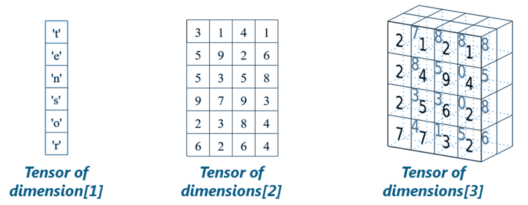
\includegraphics[width=\textwidth]{Tensor}
	   	\caption{ Tensor Matrisleri \cite{devhunter2018}}
	   	\label{Tensor}
	   \end{figure}
\subsubsection*{3.1.2 Keras}
	Keras, Python'da yazılmış ve derin öğrenme için üst düzey bir kütüphane olarak inşa edilmiştir. Theano ve TensorFlow gibi alt yapıları kullanarak, çeşitli derin öğrenme modellerini oluşturmak için temiz ve kullanışlı bir arayüz sunar. Keras, sinir ağlarının geliştirilmesi ve test edilmesi için en yaygın kullanılan üst düzey sinir ağları API'lerinden biri haline gelmiştir.\newline
	
	\clearpage
	Keras, kolay ve hızlı yöntemlerle model oluşturulmasına imkân sağlamaktadır. Bu özelliği ile yeni başlayanlar için modellerde, neler değiştirildiğinde nasıl bir etki yaratacağı deneme-yanılma yolu ile öğrenilmektedir.
	Modelleri merkezi işlem birimi (CPU) ve grafik işlemlerini yürüten işlemcileri (GPU) kullanarak sorunsuz biçimde çalıştırmaktadır. Bu şekilde istenildiği zaman işlemlerin GPU’da yapılarak zaman kazanılmasına destek olmaktadır.
	Bilgisayarlı görme modelleri olan evrişimsel sinir ağları CNN (Convolutional Neural Network) ve yinelemeli sinir ağlarını RNN (Recurrent Neural Network) desteklemektedir.
	İçerisinde kütüphane ile ilgili çok fazla kaynağın olması, oluşan ya da oluşabilecek sorunların yanıtına hızlı erişim imkânı sunmaktadır.
	
	\begin{figure}[!h]
		\centering
		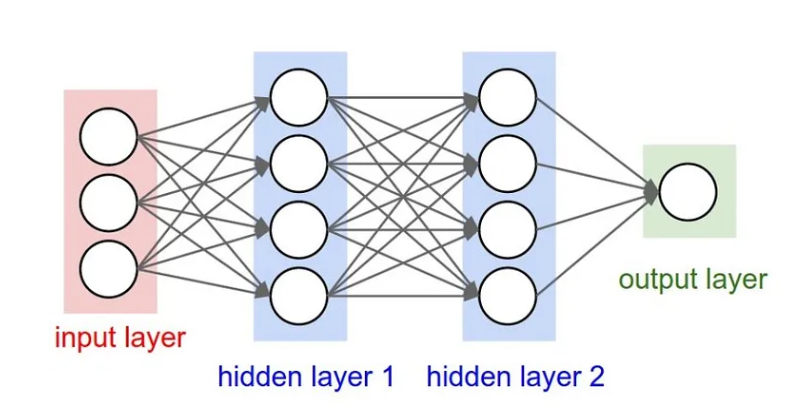
\includegraphics[width=\textwidth]{keras}
		\caption{ Keras Hidden Layer Örneği  \cite{allibhai}}
		\label{Keras}
	\end{figure}
	
		\subsubsection*{3.1.2 PyTorch}
		
		PyTorch, Torch kütüphanesine dayanan açık kaynaklı bir makine öğrenme kütüphanesidir, bilgisayarla görme ve doğal dil işleme gibi uygulamalar için kullanılır. Öncelikle Facebook'un AI Araştırma laboratuvarı tarafından geliştirilmiştir. Grafik işlem birimlerinin gücünü kullanan derin öğrenme modelleri oluştururken kullanılan bir Python kütüphanesidir.
		
		Güçlü GPU hızlandırma desteğiyle tensör hesaplamaları ve teyp tabanlı bir otograd sistemlerinde derin sinir ağları oluşturmaktır. PyTorch’un başarısının arkasındaki temel nedenlerden biri, tamamen Pythonic olması ve sinir ağ modellerini sorunsuz bir şekilde oluşturabilmesidir.
		
		Projelerin içerisinde grafik işlem birimlerini kullanan PyTorch, yapısı gereği sağladığı esneklik ve hız ile de günümüzde oldukça popüler konumdadır\cite{talentgrid_pytorch}.
		
		\subsubsection{Pythonic in nature:} Pythonic olan bu kütüphane(kodun düzenli ve temiz olması), Python veri bilimi ile kullanılır.
	
	
	\subsubsection{Hesaplamalı grafikler:} PyTorch, dinamik hesaplama grafikleri sunan bir platform sağlar, bu sayede çalışma esnasında değiştirme özelliğine sahiptir.
	
	
	PyTorch, birçok yaygın derin öğrenme modelinin uygulanmasını kolaylaştıran geniş bir model koleksiyonu olan "TorchVision" ve dil modelleri, görüntü sınıflandırma, nesne tespiti ve diğer çeşitli görevler için önceden eğitilmiş model koleksiyonu olan "TorchHub" gibi ek modüllerle birlikte gelir\cite{comert_pytorch}.
		
		\begin{table}[!h]
			\centering
			\caption{Keras-Tensorflow-PyTorch karşılaştırma tablosu.}
			\renewcommand{\arraystretch}{3.5} % Satır aralığını ayarla
			\resizebox{\textwidth}{!}{%
				\begin{tabular}{|c|c|c|c|}
					\hline
					& \includegraphics[width=2.5cm]{keras1} & \includegraphics[width=5.5cm]{tensorflow} & \includegraphics[width=3.5cm]{pytorch} \\
					\hline
					\Huge Api Düzeyi & \Huge üst düzey API & \Huge Hem yüksek hem de düşük seviyeli API'ler & \Huge Alt düzey API \\ \hline
					\Huge Hız & \Huge Yavaş & \Huge Yüksek & \Huge Yüksek \\ \hline
					\Huge Mimari & \Huge Basit, daha okunabilir & \Huge Kullanımı pek kolay değil & \Huge Karmaşık \\ \hline
					\Huge Hata Ayıklama & \Huge Hata ayıklamaya gerek yok & \Huge Hata ayıklamanın zor olması & \Huge İyi hata ayıklama yetenekleri \\ \hline
					\Huge Veri Kümesi Uyumluluğu & \Huge Yavaş ve Küçük & \Huge Hızlı ve büyük & \Huge Yüksek hız ve büyük veri kümeleri \\ \hline
					\Huge Popülarite Sıralaması & \Huge -  & \Huge - & \Huge - \\ \hline
					\Huge Benzersizlik & \Huge Çoklu arka uç desteği & \Huge Nesne Algılama İşlevselliği & \Huge Esneklik ve Kısa Eğitim Süresi \\ \hline
					\Huge Oluşturan/Sahibi & \Huge Tek başına bir kütüphane değil & \Huge Google tarafından oluşturuldu & \Huge Facebook tarafından oluşturuldu
					\\ \hline
					\Huge Kullanım Kolaylığı & \Huge Kullanıcı dostu & \Huge Kapsamlı olmayan API & \Huge Python dili ile entegre
					\\ \hline
					\Huge Kullanılan Hesaplamalı Grafikler & \Huge Statik grafikler & \Huge Statik grafikler & \Huge Dinamik hesaplama grafikleri
					\\ \hline
				\end{tabular}%
			}
		\end{table}
		
	\subsection{CNN NEDİR ?}
	 CNN genellikle görüntü işlemede kullanılan ve girdi olarak görselleri alan bir derin öğrenme algoritmasıdır. Farklı operasyonlarla görsellerdeki featureları (özellikleri) yakalayan ve onları sınıflandıran bu algoritma farklı katmanlardan oluşmaktadır. Convolutional Layer, Pooling ve Fully Connected olan bu katmanlardan geçen görsel, farklı işlemlere tabii tutularak derin öğrenme modeline girecek kıvama gelir.\newline
	
	\subsubsection{Evrişimsel Katman (Convolutional Layer)}
	
	Convolutional (evrişim katmanı) CNN algoritmalarında görüntüyü ele alan ilk katmandır. Bilindiği üzere görseller aslında içlerinde belirli değerler taşıyan piksellerden oluşan matrislerdir. Evrişim katmanında da orijinal görsel boyutlarından daha küçük bir filtre görselin üzerinde gezer ve bu görsellerden belirli özellikleri yakalamaya çalışır.
	\clearpage
	\begin{figure}[!h]
		
		\raggedright
		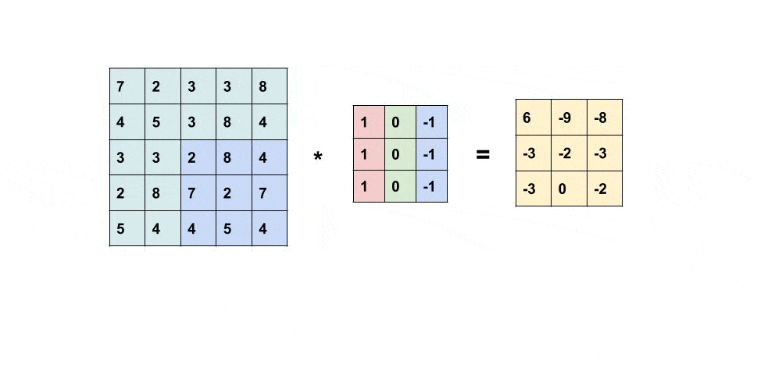
\includegraphics[width=\textwidth]{evrisimsel}
		\caption{Evrisimsel temsili resim \cite{bozkurt2021cnn}}
		\label{evrisimsel}
	\end{figure}
	
	Yukarıda şekil: \ref{evrisimsel} görüldüğü üzere 3×3’lük bir filtre, 5×5’lik bir görsel üzerinde gezdiriliyor. Çıkan sonuçlar eşitliğin sağ tarafındaki yeni matrisimiz olan feature map üzerine yazılıyor.\newline
	
	\subsubsection{Max-Pooling}
	
	evrişimli sinir ağlarında (convolutional neural networks - CNNs) kullanılan bir katman türüdür. Evrişimli sinir ağlarında, görüntü işleme gibi görsel veriler üzerinde çalışırken, boyut azaltma ve özellik çıkarma için kullanılır.\newline
	
	
	Max pooling katmanı, girdi olarak aldığı bir bölgenin (örneğin, bir pencere veya filtre) en büyük değerini çıkararak boyut azaltma işlemi gerçekleştirir. Bu, girdinin belirli bir özellikleri öne çıkararak öznitelik haritasının boyutunu azaltmaya ve işlemin hesaplama yükünü azaltmaya yardımcı olur.\newline
	
		
	Örneğin, 2x2 boyutunda bir pencereyi (genellikle 2x2 piksel) alıp, bu pencerenin içindeki en büyük değeri alarak çıktı olarak kullanır. Bu işlem, görüntünün boyutunu yarıya indirirken önemli özelliklerin korunmasına yardımcı olur. Bu tür katmanlar genellikle ardışık evrişim katmanları arasında kullanılır ve daha sonraki tam bağlantılı (fully connected) katmanlar için girdi boyutunu azaltır. Bu şekilde, ağın daha hızlı öğrenmesine ve daha fazla genelleme yeteneğine sahip olmasına yardımcı olur.
	\begin{figure}[!h]
		\centering
		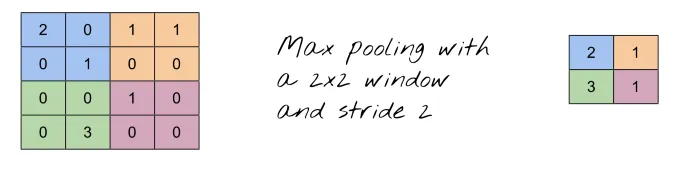
\includegraphics[width=\textwidth]{maxpooling}
		\caption{maxpooling \cite{bozkurt2021cnn}}
		\label{maxpooling}
	\end{figure}
	
	\subsubsection{Tamamen Bağlantılı Katman ve Evrişimsel Katman}
	
	bağlı katman (fully connected layer), genellikle çok katmanlı yapay sinir ağlarında bulunan bir katman türüdür.CNN'lerde, tamamen bağlı katmanlar genellikle ağın sonunda bulunur. Evrişim ve havuzlama katmanlarından sonra, elde edilen özellik haritaları, tamamen bağlı katmanlara bağlanarak sınıflandırma veya regresyon gibi görevler için kullanılır.\newline
	
	\begin{figure}[!h]
		\centering
		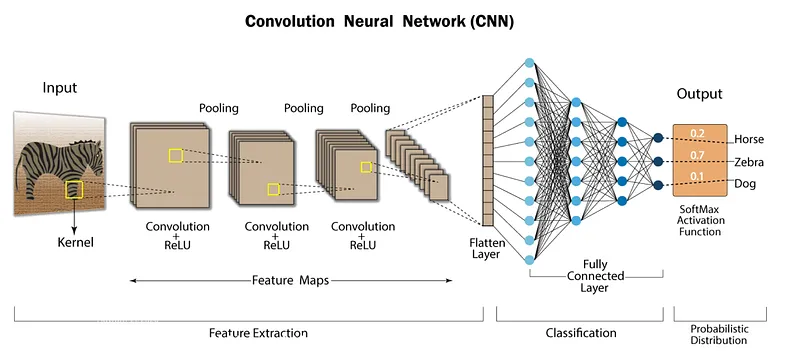
\includegraphics[width=\textwidth]{CNNArchitecture}
		\caption{ Örnek Convolutional Neural Network — CNN architecture \cite{shahriar2023cnn}}
		\label{CNNArchitecture}
	\end{figure}
	
	
	\subsection{CLIP NEDİR ?}
	CLIP-EBC (Contrastive Language-Image Pretraining with Enhanced Blockwise Classification) yönteminin kalabalık sayımı görevinde nasıl kullanıldığını açıklamaya yöneliktir.
	
	CLIP, OpenAI tarafından geliştirilen ve görüntü-tanımda üstün performans gösteren bir makine öğrenimi modelidir. CLIP, görsellerle ilgili doğal dil açıklamalarını kullanarak önceden eğitilmiş bir modeldir ve sıfırdan öğrenme yeteneğiyle bilinir. Sıfırdan öğrenme, modelin daha önce hiç görmediği kategorileri tanıyabilmesi anlamına gelir.
	\subsubsection{Sıfır Atışlı Öğrenme Nedir ve Nasıl Çalışır}
	Modelin öğrenmek üzere eğitildiği kategorilerin etiketlenmiş örneklerinin yokluğunda, sıfır atışlı öğrenme(ZSL) problemleri yardımcı bilgileri kullanır : metinsel açıklamalar, nitelikler, gömülü gösterimler veya eldeki göreve ilişkin diğer anlamsal bilgiler.\newline
	
	
	Denetimli öğrenmede ve birkaç adımlı öğrenmede (Few-Shot Learning-FSL) model, her sınıfın bir veya daha fazla etiketli örneğini doğrudan gözlemleyerek farklı sınıfları tanımayı öğrenir. Onlara rehberlik edecek bu açık ek açıklamalar olmadan, sıfır adımlı öğrenme, etiketin anlamının daha temel bir şekilde anlaşılmasını gerektirir. \newline
	
	
	
	Basit bir benzetme yapmak gerekirse, bir çocuğun bir kuşun neye benzediğini öğrenmek istediğini düşünün. Denetimli öğrenmeye veya FSL'ye benzeyen bir süreçte çocuk, hayvan resimlerinden oluşan bir kitaptaki "kuş" etiketli resimlere bakarak öğrenir. İlerlediğinde, daha önce gördüğü kuş resimlerine benzediği için bir kuşu tanıyacaktır. Ancak ZSL senaryosunda bu tür etiketli örnekler mevcut değildir. Bunun yerine çocuk, kuşlarla ilgili bir ansiklopedi maddesini okuyabilir ve onların havada uçabilen tüyleri, gagaları ve kanatları olan küçük veya orta boy hayvanlar olduğunu öğrenebilir. Daha sonra daha önce hiç görmemiş olmasına rağmen gerçek dünyadaki bir kuşu tanıyabilecektir çünkü kuş kavramını öğrenmiştir.\newline
	\subsubsection{Transfer öğrenim}
	
	Eğitim için gereken zaman ve kaynakların yanı sıra görünmeyen sınıfları tanımlamak için gereken yardımcı bilgi miktarını en aza indirmek amacıyla ZSL, modelleri sıfırdan eğitmek yerine  genellikle transfer öğrenmeden (eğitilmiş bir modelin yeni bir görev için yeniden kullanılması) yararlanır.\newline
	
	Transfer öğrenimi, sınıfları ve örnekleri anlamsal yerleştirmeler olarak temsil eden ZSL yöntemlerinde belirgin bir şekilde kullanılır . Örneğin, sıfır atışlı metin sınıflandırması gerçekleştiren bir model, kelimeleri vektör yerleştirmelerine dönüştürmek için zaten çok sayıda dil verisi üzerinde önceden eğitilmiş transformatör tabanlı bir model kullanabilir. Benzer şekilde, sıfır atışlı bir görüntü sınıflandırma modeli, ResNet veya U-Net gibi önceden eğitilmiş bir evrişimli sinir ağını (CNN) yeniden tasarlayabilir , çünkü sınıflandırmayı bilgilendirebilecek önemli görüntü özelliklerini belirlemeye yardımcı olan filtre ağırlıklarını zaten öğrenmiş olacaktır.\newline
	
	Transfer öğrenimi, modelin görülen sınıflara ilişkin bilgisinin, görünmeyen sınıflara ilişkin yardımcı bilgi olarak kullanılabileceği Genelleştirilmiş sıfır vuruşlu öğrenme (GSZL) için özellikle önemlidir. Örneğin, bir nesne algılama modelinin boz ayıları tanımayı zaten öğrendiğini hayal edin. Kutup ayılarının etiketli örneklerini vererek onu kutup ayılarını tanıması için eğitmek yerine, kutup ayılarının beyaz kürklü boz ayılara benzediğini anlayacak şekilde eğitilebilir\cite{bergmann2024zero}.\newline
	
	
	Zero-shot learning, bir modelin eğitim sırasında hiç görmediği sınıfları tanımayı veya bu sınıflara ait özellikleri öğrenmeyi amaçlayan bir makine öğrenimi yaklaşımıdır. Bu senaryoda, verilen bilgilere dayanarak Aşağıdaki resimlerden hangi resmin "gavyal" olduğunu tahmin etmeye çalışalım.
	
		\begin{landscape} % Rotating the page
		
		
		\begin{figure}[!h] % Use [p] to place the figure on a separate page
				Verilen bilgiler doğrultusunda seçim yapınız.\newline "Yakalanan en büyük gavyal 7 m. uzunluğunda idi, ama normalde uzunlukları 5 metreyi geçmez."
			"Balık yakalama yönünde evrimleşmiş uzun ve dar ağız yapısı"
			"Gavyal, tuzlu su timsahından sonra dünyanın en büyük timsah çeşididir."
			
			\begin{minipage}[t]{0.400\linewidth}
				\centering
				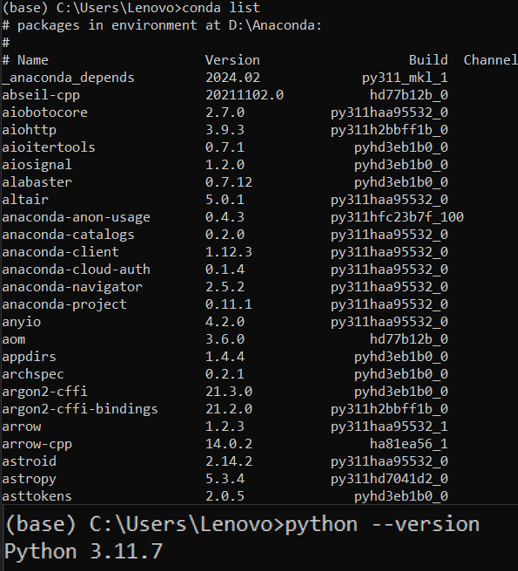
\includegraphics[width=\linewidth]{Resim1}
				\caption{\cite{ceylan2014hayvanlar}}
			\end{minipage}\hfill
			\begin{minipage}[t]{0.400\linewidth}
				\centering
				\includegraphics[width=\linewidth]{Resim2}
				\caption{\cite{ceylan2014hayvanlar}}
			\end{minipage}
			
			\vspace{0.5cm}
			
			\begin{minipage}[b]{0.400\linewidth}
				\centering
				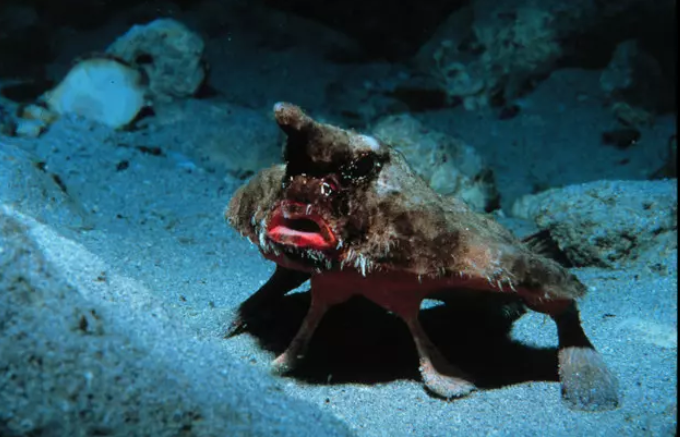
\includegraphics[width=\linewidth]{Resim3}
				\caption{\cite{ceylan2014hayvanlar}}
			\end{minipage}\hfill
			\begin{minipage}[b]{0.400\linewidth}
				\centering
				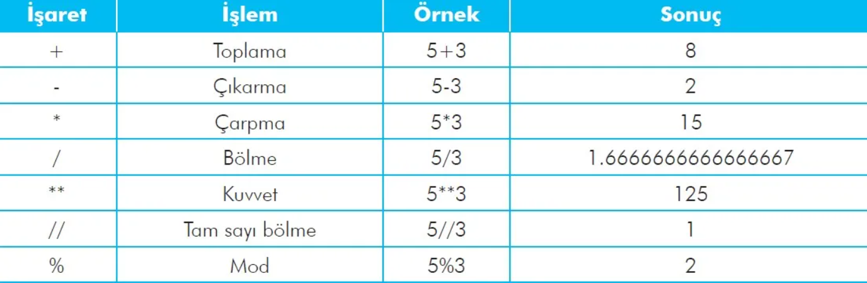
\includegraphics[width=\linewidth]{Resim4}
				\caption{\cite{stokfoto}}
			\end{minipage}
			
		\end{figure}
		
	\end{landscape}
	
	
		Bu bilgilere dayanarak, en büyük olasılıkla gavyal resminin 4. olduğunu söyleyebilirim. Çünkü 3. bilgi, diğerlerine göre daha spesifik bir özellik veriyor ve gavyalın  tuzlu su timsahından sonra dünyanın en büyük timsah çeşididir belirtiyor. Dolayısıyla, bütün  resimler arasında seçim yaparken, bu bilgiyi göz önünde bulundurarak 4. resmin gavyal olma olasılığının daha yüksek olduğunu düşünüyorum. Bu nedenle, gavyal resminin 4. olduğunu tahmin ederdim.
	
	
	\subsection{Geliştirilmiş Blok Bazında Sınıflandırma}
	
		Geleneksel yöntemler blok bazlı regresyona dayanmaktadır. Ancak, bu Geliştirilmiş Blok Bazında Sınıflandırma (Enhanced Blockwise Classification (EBC)) çerçevesi, her blok içindeki sayı değerini birkaç önceden tanımlanmış aralığa sınıflandırmayı amaçlayan bir fikre dayanmaktadır. Geliştirme, üç ana noktadan gelmektedir: ayrıklaştırma politikası, etiket düzeltme ve kayıp fonksiyonu\cite{idrees2018composition}.
	\newline  
	
	
	Bu yöntem, görüntüyü küçük bloklara böler ve her bir bloktaki nesne sayısını belirli bir aralığa sınıflandırmayı amaçlar. Bu sınıflandırma, belirli bir blok içindeki nesne sayısını tahmin etmeye odaklanır ve nesnelerin yoğunluğunu ölçmek için kullanılır.
	\newline   
	
	
	Ayrıklaştırma Politikası: EBC'de kullanılan ayrıklaştırma politikası, nesne sayısını belirli aralıklara sınıflandırmak için belirlenen stratejiyi ifade eder. Bu strateji, nesnelerin dağılımını en iyi şekilde yansıtmak için dikkatlice seçilir.
	
	Etiket Düzeltme: EBC, doğru etiketleme için bir düzeltme mekanizması içerir. Bu mekanizma, modelin öğrenirken daha doğru sonuçlar elde etmesine yardımcı olur ve modelin performansını artırır.
	
	Kayıp Fonksiyonu: EBC'nin kayıp fonksiyonu, modelin eğitilirken hata miktarını belirlemek için kullanılır. Bu kayıp fonksiyonu, modelin en iyi sınıflandırma sonuçlarını üretmek için optimize edilir.
	
	Bu üç bileşen, EBC'nin geliştirilmiş performansını sağlar ve nesne sayımı gibi görevlerde daha etkili bir şekilde çalışmasını sağlar.
	
	\begin{figure}[!ht]
		\subcaptionsetup{labelformat=empty}
		\raggedright
		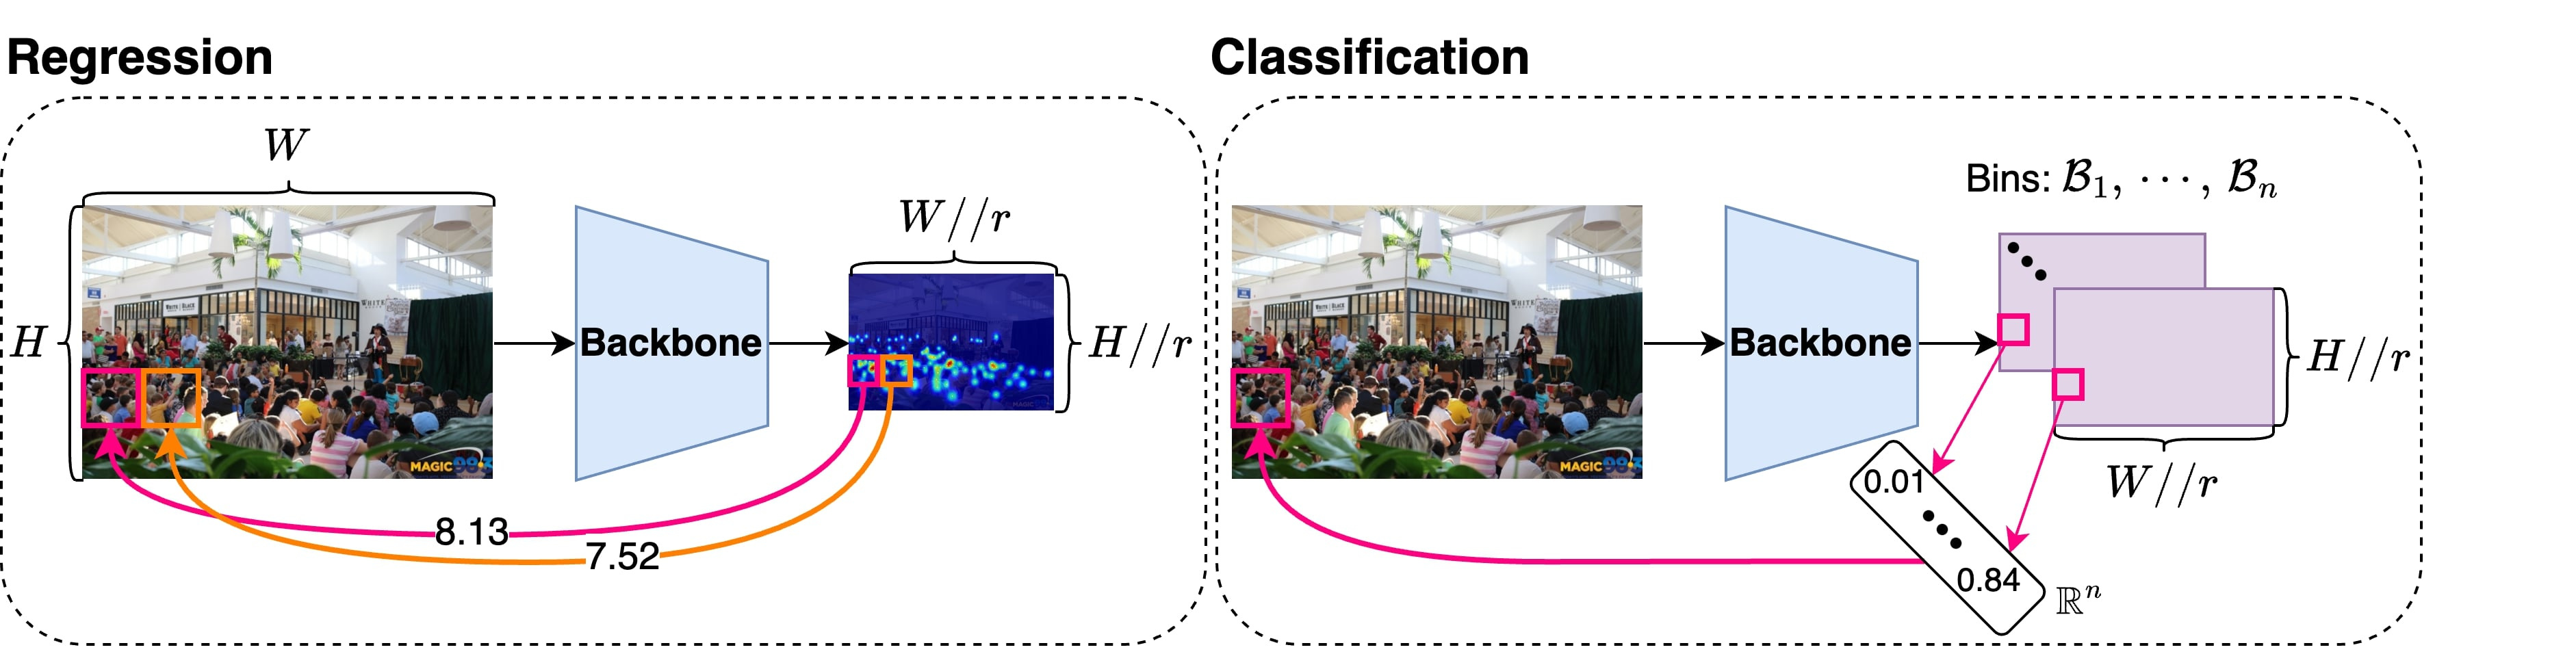
\includegraphics[width=\textwidth]{regression1}
		\caption{EBC \cite{idrees2018composition}}
		\label{Ornek_sonuc1}
	\end{figure}
	\clearpage
\begin{landscape} % Sayfayı döndürme
	
	\begin{figure}[p]
		\centering
		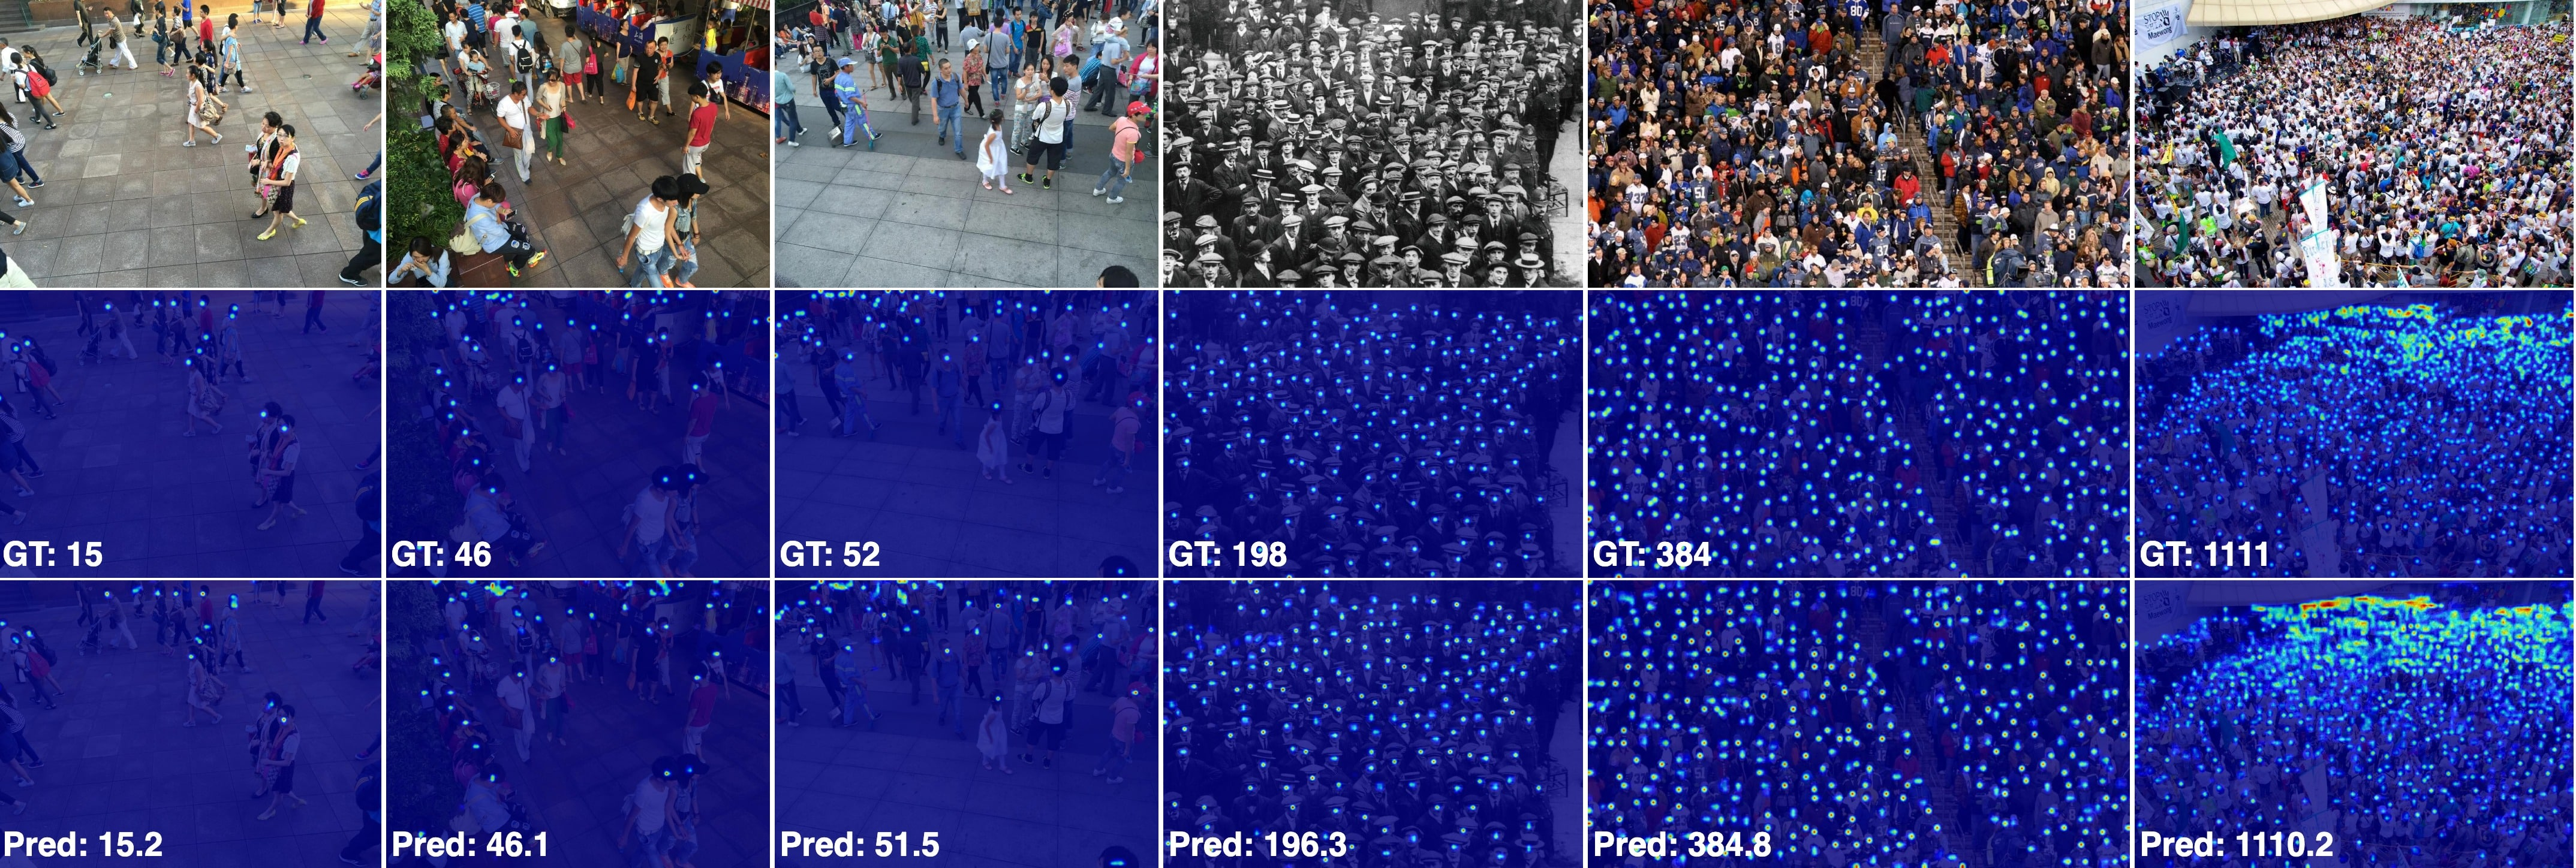
\includegraphics[height=0.65\textheight]{visualization} % Yüksekliği sayfa yüksekliğinin 8/10'u olarak ayarla
		\caption{Proje Çıktısı Örneği \cite{ma2024clip}.}
	\end{figure}
	
\end{landscape}
	
\end{justify}
\subsection*{3 C-CNN}
\begin{justify}
 Contourlet CNN, görüntü işleme ve analizinde kullanılan bir derin öğrenme mimarisidir. Özellikle \textcolor{red}{doku analizi ve nesne tanıma} gibi alanlarda oldukça etkilidir. Contourlet dönüşümü(Contourlet Dönüşümü görüntülerin yumuşak bölgelerinin sınırlarında karşılaşılan kenar yumuşaklıklarını saptamada daha başarılıdır\cite{konuk2016hyperspectral}.) adı verilen bir matematiksel işlemi kullanarak görüntüyü farklı ölçeklerde ve yönlerde analiz eder ve bu analizleri konvolüsyonel sinir ağları ile birleştirerek karmaşık desenleri ve nesneleri öğrenir.\newline
 
 

Contourlet CNN'in Avantajları:
Çok Ölçekli Analiz: Görüntüleri farklı ölçeklerde analiz ederek, hem genel doku bilgilerini hem de ince ayrıntıları yakalayabilir.
Yönsel Duyarlılık: Görüntüdeki doku ve nesnelerin yönünü de dikkate alarak daha kapsamlı bir analiz yapabilir.
Derin Öğrenme Gücü: Konvolüsyonel sinir ağları ile öğrenerek, karmaşık desenleri ve nesneleri yüksek doğrulukla tanıyabilir.\newline

Contourlet CNN'in Kullanım Alanları:
Doku Analizi: Tıbbi görüntülerde doku anormalliklerini tespit etme, dokuların türünü ve özelliklerini sınıflandırma.
Nesne Tanıma: Fotoğraflarda ve videolarda nesneleri (insanlar, araçlar, hayvanlar vb.) algılama ve sınıflandırma.
Görüntü Sınıflandırma: Görüntüleri (doğal manzaralar, şehir manzaraları, iç mekanlar vb.) kategorilere ayırma.
Görüntü Geliştirme: Görüntülerdeki gürültüleri azaltma, keskinleştirme, kenar algılama.\newline


\raggedright maoz ragab'ın projesinden yararlanılmıştır\cite{ragab2021crowdcounting}.\newline

yavisankar Crowd-Counting-Problem projesinden yaralanılmıştır\cite{githubproject}.
\end{justify}


\clearpage


\section{BULGULAR VE TARTIŞMA}
	
\rule{\linewidth}{0.65pt}

\begin{Verbatim}
[--weight_decay WEIGHT_DECAY]
[--warmup_epochs WARMUP_EPOCHS] [--warmup_1r WARMUP_LR]
[--total_epochs TOTAL_EPOCHS] [--eval_start EVAL_START]
[--eval_freq EVAL_FREQ] [--num_workers NUM_WORKERS]
[--local_rank LOCAL_RANK] [--seed SEED]
trainer.py: error: the following arguments are required: --dataset
An exception has occurred, use %tb to see the full traceback.
SystemExit: 2	
\end{Verbatim}
	
\centering \textbf{Kod Bloğu: Proje hataları 1} 

\begin{justify}
Projenin Linux ortamında yazılmış olması nedeniyle, Windows ortamında .sh dosyaları çalışmamaktadır. Bu durumda, Windows ortamında projenin çalışması için .sh dosyasından alınan dataset parametresini manuel olarak girilmesi gerekmektedir.
\end{justify}

\rule{\linewidth}{0.65pt}
\begin{verbatim}
def standardize\_dataset\_name {(dataset: str) -> str:}
assert dataset.lower() in available_datasets, f"Dataset {dataset}
is not available."
if dataset.lower() in ["shanghaitech_a", "sha"]:
return "sha"
elif dataset.lower() in ["shanghaitech_b", "shb"]:
return "shb"
elif dataset.lower() in ["ucf_qnrf", "qnrf", "ucf-qnrf"]:
return "qnrf"
elif dataset.lower() in ["nwpu", "nwpu_crowd", "nwpu-crowd"]:
return "nwpu"
else: # dataset.lower() in ["jhu", "jhu_crowd", "jhu_crowd_v2"]
return "jhu"
\end{verbatim}
\centering \textbf{Kod Bloğu: Proje hataları 2} 
\begin{justify}
	
Proje hataları 1, kodunun hata devamı olarak görülebilir. Projenin başlatılması sırasında ilgili parametrelerin otomatik olarak çekilmemesi nedeniyle devam eden bir sorun olarak görülebilir. Bu durumda, ilgili parametrelerin değerlerini manuel olarak  kodun ilgili bölümüne girmek gerekmektedir.
\end{justify}


\rule{\linewidth}{0.65pt}
\begin{verbatim}
File ~/Documents/CLIP-EBC-main/utils/train_utils.py:63 in get_loss_fn
assert args.weight_ot is not None and args.weight_tv is not None, 
"weight_ot and weight_tv cannot be None when bins is None."	
AttributeError: 'Namespace' object has no attribute 'weight_ot'
\end{verbatim}
\centering \textbf{Kod Bloğu: Proje hataları 3}	
\begin{justify}	
	Proje hataları 1, kodunun hata devamı olarak görülebilir. Projenin başlatılması sırasında ilgili parametrelerin girilmemiş olduğu farkedilip Manuel olarak değerler girilmiştir.
\end{justify}

\rule{\linewidth}{0.65pt}
\begin{verbatim}
required=True ifadesini  required=False\end{verbatim} olarak değiştirmek, betiğinizi esnek hale getirir. Artık argümanlar zorunlu değil, yani kullanıcılar bunları belirtmek zorunda değiller. Eğer belirtilmezse, kod varsayılan bir değer kullanır.

\begin{verbatim}
ap.add_argument("-f", required=False)	\end{verbatim}
\begin{justify}
ifadesi ise Jupyter Notebook veya diğer not defteri uygulamalarında argparse'ın özel bir durumunu ele alıyor. -f argümanı, Jupyter Notebook'un kendi ihtiyaçları için kullanılır ve eğer belirtilmezse, kod hata vermez.\newline


Bu değişiklikler, betiğinizi veya modülünüzü Jupyter Notebook veya diğer not defteri uygulamalarında daha rahat ve sorunsuz bir şekilde kullanmanızı sağlar. Kullanıcılar istediklerinde argümanları belirtebilirler, belirtmezlerse kod varsayılanları kullanır ve hata almazlar\cite{CB_Acnt}.
\end{justify}
\rule{\linewidth}{0.65pt}

\begin{verbatim}
File c:\users\bakid\onedrive\belgeler\clip-ebc-main\datasets\crowd.py:11
from .utils import get_id, generate_density_map	
ImportError: attempted relative import with no known parent package \newline
\end{verbatim}
\begin{justify}
	Proje sahibi tarafından belirtilen gereksinimlere göre, ilgili kod bölümlerindeki eksiklikler tespit edilmiş ve gerekli düzeltmeler yapılmıştır.
\end{justify}
\rule{\linewidth}{0.65pt}

	\subsubsection{Cuda Sürüm Uyumsuzlukları Ve DDU}

\begin{justify}
	CUDA (Compute Unified Device Architecture), GPU (Graphics Processing Unit) için NVIDIA'nın sunduğu C programlama dili üzerinde eklenti olarak kullanıma sunulan bir mimari ve teknolojidir\cite{wiki:CUDA}.
\end{justify}	
	
	
		\subsubsection{Ekran Sürücüsü Kaldırıcı(DDU) NEDİR ?}
	\begin{justify}
			Ekran Sürücüsü Kaldırıcı bilgisayarda yer alan ekran kartı(Nvidia,AMD) sürücüsü veya sürücülerinin kaldırılmasını sağlayan bir program/uygulamadır.
		indirip kullandığım sürüm Display Driver Uninstaller (DDU) download version 18.0.7.6\cite{DDU}.\newline
	\end{justify}
\clearpage

\lstset{breaklines=true, breakatwhitespace=true, basicstyle=\ttfamily}

\begin{lstlisting}
	v2.2.1
	Conda
	OSX
	# conda
	conda install pytorch=2.2.1 torchvision==0.17.1 torchaudio==2.2.1 -c pytorch
	Linux and Windows
	# CUDA 11.8
	conda install pytorch==2.2.1 torchvision==0.17.1 torchaudio==2.2.1 pytorch-cuda-11.8c pytorch -c nvidia
	# CUDA 12.1
	conda install pytorch==2.2.1 torchvision==0.17.1 torchaudio==2.2.1 pytorch-cuda 12.1 c pytorch -c nvidia
	# CPU Only
	conda install pytorch=2.2.1 torchvision==0.17.1 torchaudio==2.2.1 cpuonly pytorch
	Wheel
	OSX
	pip install torch==2.2.1 torchvision==0.17.1 torchaudio==2.2.1
	Linux and Windows
	# ROCM 5.7 (Linux only)
	pip install torch==2.2.1 torchvision==0.17.1 torchaudio=2.2.1 --index-url https://download.pytorch.org/whl
	# CUDA 11.8
	pip install torch==2.2.1 torchvision==0.17.1 torchaudio==2.2.1 --index-url https://download.pytorch.org/whl
	# CUDA 12.1
	pip install torch==2.2.1 torchvision==0.17.1 torchaudio=2.2.1 --index-url https://download.pytorch.org/whl
	# CPU only
	pip install torch==2.2.1 torchvision==0.17.1 torchaudio==2.2.1 --index-url https://download.pytorch.org/whl
\end{lstlisting}



\begin{landscape} % Sayfayı döndürme
	
	\begin{figure*}[p]
		\centering
		\includegraphics[width=\linewidth]{CUDA-Pytorch}
		\caption{CUDA-Pytorch \cite{pytorch}.}
	\end{figure*}
	
	
\end{landscape}
	
\clearpage
\rule{\linewidth}{0.65pt}	
\begin{verbatim}
packages spyder_kernels\py3compat.py:356 in compat_exec
exec(code, globals, locals)
File c:\users\bakid\onedrive\belgeler\clip-ebc-main7\trainer.py:1
import torch
File ~\anaconda3\Lib\site-packages\torch\__init__.py:21
from torch import _C
ImportError: DLL load failed while importing _C: Belirtilen modül bulunamadı.
\end{verbatim}
\centering\textbf{DLL hatası}\newline
	
	\begin{justify}
			Pytorch 2.3.0 sürümü uninstall edilip önerilen sürüm 2.2.1 sürümü tekrardan yüklenilmiş ve DLL sorunu ortadan kaldırılmıştır.
	\end{justify}

	

\rule{\linewidth}{0.65pt}
\begin{justify}
	\begin{verbatim} get_model
		return vanilla_clip(
		File\OneDrive\Belgeler\CLIP-EBC-main7\models\clip\model.py:165 in_vanilla_clip
		return VanillaCLIP(
		File ~\OneDrive\Belgeler\CLIP-EBC-main7\models\clip\model.py: 57
		in_init
		self.anchor_points = torch.tensor (anchor_points, dtype=torch.float32,
		 requires_grad=False).view (1, -1, 1, 1)
		TypeError: must be real number, not NoneType
	\end{verbatim}
	\hspace{-2em} % Metni 2 em birim sola yaslar

	Anchor\_points hatası veriyor boş değer dönüyordu devamında aşağıdaki kod parçası denenmiş ve olumlu sonuç vermiştir.\newline
	
	
	\begin{verbatim}
		self.bins bins
		if anchor_points is not None:
		self.anchor_points = torch.tensor(anchor_points, dtype=torch.float32, 
		requires_grad=False).view(1, -1, 1, 1)
		print(anchor_points)
		else:
		print(anchor_points)
		return #anchor_points'in None olduğu durumu yönetin
		(örneğin,varsayılan bir değer ayarlayın)
	\end{verbatim}
	\hspace{-1em} Daha sonraki denemelerde 
	\begin{verbatim}
		self.bins bins
		self.anchor_points = torch.tensor (anchor_points, dtype=torch.float32, 
		requires_grad=False).view(1, -1, 1, 1) print(anchor_points)
	\end{verbatim}
	\hspace{-1em}	kodunun çalıştığı gözlemlenmiştir sorun çözülmüştür.\newline
	
\end{justify}


\rule{\linewidth}{0.65pt}
\begin{verbatim}
Hata 2 : File\OneDrive\Belgeler\CLIP-EBC-main7 datasets\crowd.py:67 in __init__
self._check_sanity_()
File ~\OneDrive\Belgeler\CLIP-EBC-main7\datasets\crowd.py:114 in _check_sanity_
assert len(self.image_names) == len(self.label_names) == 300, 
f"ShanghaiTech_A train split should have 300 images, but found {len(self.image_names)}."
AssertionError: ShanghaiTech_A train split should have 300 images, but found 0.
\end{verbatim}
\textbf{Self.root(dizin bulamama hatası)}
\begin{justify}
	Hata sorunu Label\_names ve image\_names kısmında okuyamama bulamama sorunları ile alakalıdır bu sorun ise Self.root methodunu ilgilendirmektedir.
\end{justify}
\rule{\linewidth}{0.65pt}


	\begin{verbatim}
print(f"Rank {Local_rank} process among (nprocs) processes.") 
def run(local_rank: int, nprocs: int, args: ArgumentParser) -> None:
init_seeds(args.seed + local_rank) 
setup(local_rank, nprocs) 
print(f"Initialized successfully. Training with {nprocs} GPUs.") 
device = f"cuda: {Local_rank}" if local_rank != -1 else "cuda:0" 
print(f"Using device: {device}.") 
ddp = nprocs > 1 
if args.truncation is None: 
# regression, no truncation. bins, anchor_points = None, None 
else: 
with open(os.path.join(current_dir, "configs", 
f"reduction_{args.reduction}.json"), "r") as f: 
config = json.load(f) 
[str(args.truncation)] [args.dataset] bins = config["bins"] [args.granularity]
	
anchor_points = config["anchor_points"] [args.granularity] ["average"] 
if args.anchor_points == "c 
bins = [(float(b[0]), float(b[1])) for bin bins] 
anchor_points = [float(p) for p in anchor_points] 
args.bins = bins 
args.anchor_points = anchor_points 
model = get_model(
backbone="resnet50",
input_size=args.input_size,
reduction=args.reduction,
bins=bins,
anchor_points=anchor_points,
prompt_type=args.prompt_type
)
\end{verbatim}
\textbf{Model Hatası}\newline
Orjinalinde \texttt{backbone=args.model} olan kod parçası (Orjinal kodda "vgg19\_ae" kullanılırken bizim modelimiz "clip\_resnet50" olarak seçilmiştir) boş olarak döndüğü için manuel tanımlama yapılmıştır.


\begin{justify}
\rule{\linewidth}{0.65pt}
 	\begin{verbatim}
File\OneDrive\Belgeler\CLIP-EBC-main7\datasets\crowd.py:66 in init
self._make_dataset__()
File\OneDrive\Belgeler\CLIP-EBC-main7\datasets\crowd.py:114 in _make_dataset_
label_names.sort(key=get_id)
File ~\OneDrive\Belgeler\CLIP-EBC-main7\datasets\utils.py:8 in get_id return
	
int(name_without_extension.split("_")[1])
ValueError: invalid literal for int() with base 10: 'IMG' 
\end{verbatim}
\textcolor{red}{Hatalı kod:}
\begin{verbatim}
	def get_id(x: str) -> int:
	return int(x.split(".")[0])
\end{verbatim}\newline
\textcolor{red}{Düzeltilmiş kod:}
\begin{verbatim}
	def get_id(x: str) -> int:
	if x.endswith(".jpg"):
	name_without_extension = x.split(".")[0]
	return int(name_without_extension.split("_")[1])
	else:
	name_without_extension = x.split(".")[0]
	return int(name_without_extension.split("_")[2])
\end{verbatim}

\centering \textbf{Dosya okuma hatası}\newline

\begin{justify}
Kullanılan veri setindeki resim(.jpg) isimleri "IMG\_1" şeklinde iken 
ground-truth değerleri "GT\_IMG\_1" şeklindedir, key\_id bulma sorunu bu şekilde çözülmüştür.
\end{justify}


\begin{landscape} % Rotating the page
	
	
\begin{figure}[!h] % Use [p] to place the figure on a separate page
		\centering
		\textbf{CUDA VE GPU SEÇİMLERİ}
		
		
		\begin{minipage}[t]{0.970\linewidth}
			\centering
			\includegraphics[width=\linewidth]{smi}
			\caption{nvidia-smi terminal görüntüsü}
		\end{minipage}
		
		
		
\end{figure}
	
\end{landscape}


\begin{landscape} % Rotating the page
	
	
\begin{figure}[!h] % Use [p] to place the figure on a separate page
		\centering
		
		
		\begin{minipage}[b]{0.970\linewidth}
			\centering
			\includegraphics[width=\linewidth]{gorev-yoneticisi}
			\caption{Windows görev yöneticisi GPU seçenekleri}
		\end{minipage}\hfill
		
		
\end{figure}
	
\end{landscape}

\end{justify}


\begin{verbatim}
args: ArgumentParser,
model: nn.Module,
optimizer: Adam,
scheduler: LambdaLR,
	
) -> Tuple[nn.Module, Adam, Union[LambdaLR, None], int, \\
Union[Dict[str, float], None), Dict[str, List[float]]):
	
ckpt_path = os.path.join(args.ckpt_dir, "best_mae.pth")
print("ne buuuu kiii", args.ckpt_dir)
print("ne buuuu", ckpt_path)
\end{verbatim}
\centering \textbf{Checkpoint Hatası}
\begin{figure}[!h]
	
	\centering
	\includegraphics[width=\linewidth]{klasor}
	\caption{Klasor yapısı örneği }
	
\end{figure}

\RaggedRight \section{SONUÇ}
\begin{justify}
Bu çalışma sürecinde, CLIP-EBC yöntemiyle kalabalık sayımı alanında önemli bir ilerleme sağlanmıştır. Ancak, projenin başarılı bir şekilde tamamlanamamasının arkasında çeşitli teknik zorluklar yatmaktadır. Özellikle, grafik kartı ayarlamaları ve eğitim sürecinde karşılaşılan kodda'ki hata problemleri, CLIP modeli gibi karmaşık yapılı modellerin uygulanmasını ve verimli bir şekilde eğitilmesini engellemiştir.

Eğitim sürecinde yaşanan hatalar ve donanım sorunları, projenin ilerlemesini etkilemiş ve istenen sonuçların elde edilmesini engellemiştir. Bu durum, gelecekteki benzer çalışmalar için dikkat edilmesi gereken teknik ve altyapısal zorlukları ortaya çıkarmıştır.

Sonuç olarak, CLIP-EBC yöntemi, kalabalık sayımı alanında yeni bir metodoloji olarak önemli bir potansiyel sunmaktadır. Ancak, projenin tamamlanamamış olması, daha ileri araştırmalar için bu alanda yapılacak çalışmaların daha fazla geliştirilmesi gerektiğini göstermektedir. Bu tür yenilikçi projelerde karşılaşılan her bir zorluk, gelecekteki çalışmalar için önemli bir öğrenme deneyimi olarak değerlendirilmelidir.
\end{justify}
	
	
	
	
	\bibliographystyle{plain}
	\bibliography{references.bib} 
\end{document}